\documentclass[12pt]{article}

\newcommand{\sref}[1]{Section$\,$\ref{#1}}

\usepackage{times}
\usepackage{robbib}
\usepackage{fullpage}
\usepackage{graphicx}
\usepackage{mygb4e}
\usepackage{url}
\usepackage{multirow,xspace}

\newcommand{\tdl}{\textsc{tdl}}
\newcommand{\hpsg}{\textsc{hpsg}\xspace}
\newcommand{\itsdb}{\mbox{\sf \lbrack incr tsdb()\rbrack}}

%% TODO: Change ``Redwoods-style'' to ``dynamic'' except for
%% the first instance.


\title{From Database to Treebank:\\ On Enhancing Hypertext Grammars with
Grammar Engineering and Treebank Search}

\author{Emily M.\ Bender$^\spadesuit$, Sumukh Ghodke$^\heartsuit$,\\ Timothy Baldwin$^\heartsuit$ and Rebecca Dridan$^\clubsuit$\\
\normalsize $^\spadesuit$University of Washington, $^\heartsuit$University of Melbourne, $^\clubsuit$University of Oslo}

\date{}

\begin{document}

\maketitle

\newpage

\paragraph{Abstract}
This paper describes how electronic grammars can be further enhanced
by adding {\it machine-readable grammars} and {\it treebanks}.  We
explore the potential benefits of implemented grammars and treebanks
for descriptive linguistics, following the discursive methodology of
\namecite{Bir:Sim:03} and the values and maxims identified by
\namecite{Nordhoff:08}.  We describe the resources which we believe
make implemented grammars and treebanks feasible additions to
electronic descriptive grammars, with a particular focus on the
Grammar Matrix grammar customization system
\cite{Ben:Dre:Fok:Pou:Sal:10} and the Fangorn treebank search
application \cite{Gho:Bir:10}.  By presenting an example of an
implemented grammar based on a descriptive prose grammar, we show one
productive method of collaboration between grammar engineer and field
linguist, and propose that a tighter integration could be beneficial
to both, creating a virtuous cycle that could lead to more effective
and informative resources.

\newpage

\section{Introduction}

This paper describes how electronic grammars can be further enhanced by
adding {\it machine-readable grammars} and {\it treebanks}, or sets of
structured annotations produced by the machine-readable
grammars.\footnote{We are grateful to the audience at the Conference on
  Electronic Grammaticography and an anonymous reviewer for helpful
  discussion.  This material is based in part upon work supported by the
  National Science Foundation under Grants No.\ 0644097 and No.\
  0317826, and the Australian Research Council under Grant No.\
  DP0988242.  Any opinions, findings, and conclusions or recommendations
  expressed in this material are those of the author(s) and do not
  necessarily reflect the views of the National Science Foundation.  }
Following \namecite{Good:04}, we understand a descriptive grammar to be
a set of annotations over texts and lexicon, including both prose
descriptions and structured descriptions.  In an electronic descriptive
grammar, annotations are illustrated with exemplars drawn from the text
but are understood to express generalizations over more examples.  This
is illustrated in Figure~\ref{fig:good}, from \citeboth{Good:04}.
Machine-readable grammars can be understood as another kind of
structured description.  Because they are interpreted by computers, they
are required to achieve a higher level of consistency, with descriptions
of various phenomena integrated to form a cohesive whole
\cite{Bender:08}. Implemented grammars can automatically produce
annotations over individual examples, which can in turn be aggregated
and searched \cite{Gho:Bir:10}.  This vision is illustrated in
Figure~\ref{fig:bigpicture}.


\begin{figure}[hb]
\centering
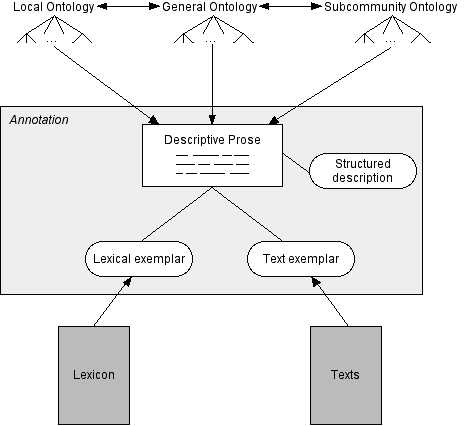
\includegraphics[width=3in]{Annotation}
\caption{The structure of an annotation \protect\cite{Good:04}}
\label{fig:good}
\end{figure}

\begin{figure}
\centering
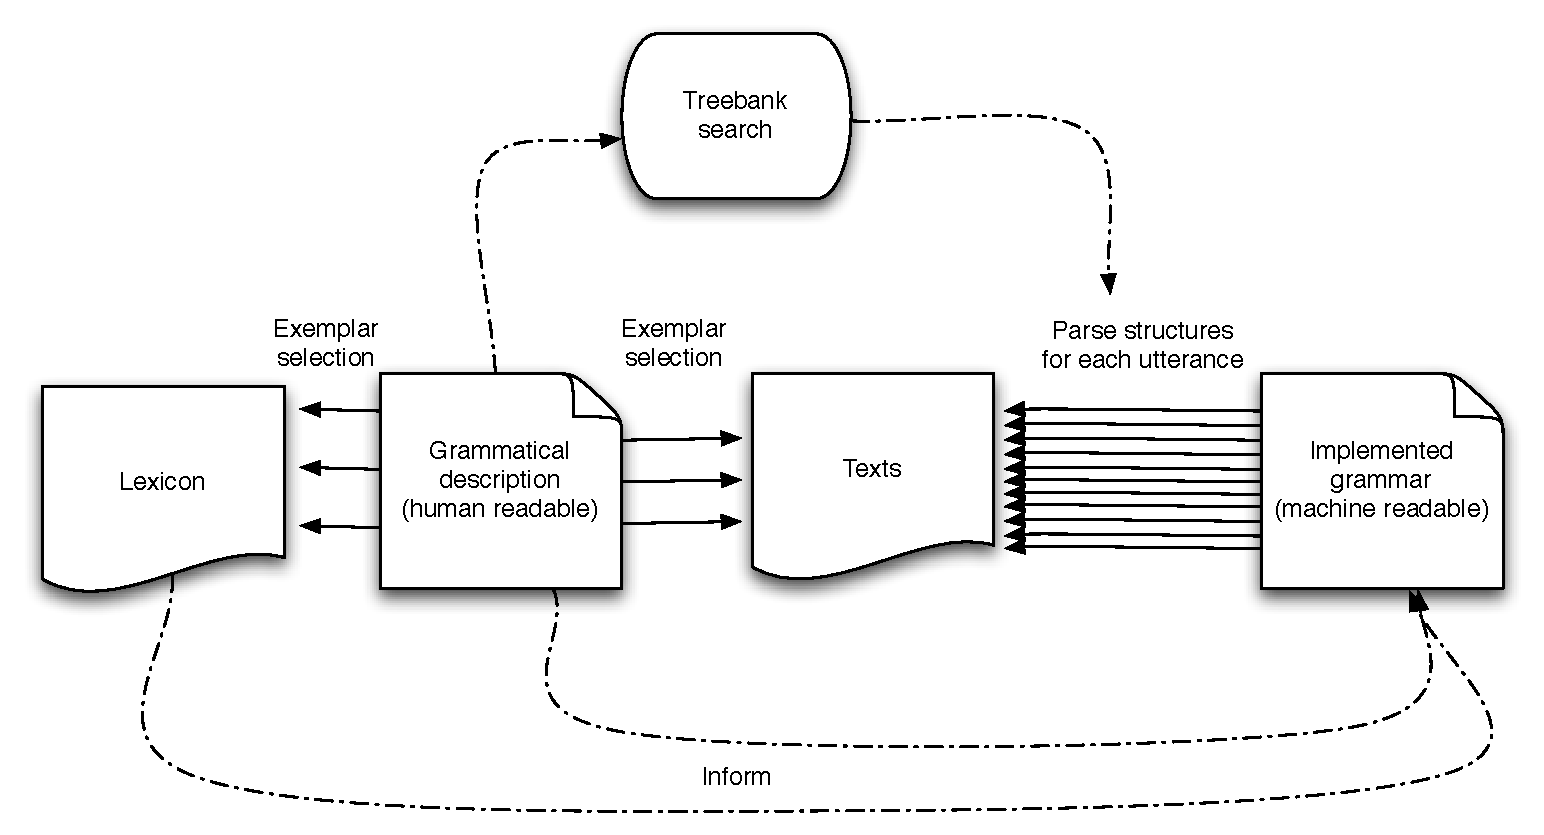
\includegraphics[width=6.5in]{BigPicture3.pdf}
\caption{Schematic view of electronic grammars with treebanks}
\label{fig:bigpicture}
\end{figure}


Our purpose in this paper is to explore the potential benefits of
implemented grammars and treebanks for descriptive linguistics and to
present to the descriptive linguistic community the currently existing
tools which can facilitate their creation.  In \sref{sec:bg}, we
describe implemented grammars and treebanks and give an example of
grammar engineering in the context of endangered languages.
\sref{sec:ts} describes treebank search, including use cases relevant
to descriptive and documentary linguistics and how it can be
integrated into an electronic descriptive grammar.  Following the
discursive methodology of \namecite{Bir:Sim:03} and the values and
maxims identified by \namecite{Nordhoff:08}, in \sref{sec:vm} we
explore the impact of augmenting descriptive grammars with treebanks.
Finally, in \sref{sec:gt} we explore the resources which we believe make
implemented grammars and treebanking feasible additions to electronic
descriptive grammars.


\section{Background}
\label{sec:bg}

\subsection{Implemented grammars}
\label{sec:wmb}

Implemented grammars are collections of linguistic rules written in a
formalism that can be interpreted by appropriate software in order to
apply those rules to linguistic inputs.\footnote{Implemented grammars
  of this sort are also descriptive in the sense that they capture
  linguistic generalizations.  For present purposes, we will use the
  phrase {\it (electronic) descriptive grammars} to refer to prose
  statements of linguistic analyses and {\it implemented grammars} or
  {\it machine-readable grammars} to refer to formal sets of rules
  that can be interpreted by a computer.}  These inputs can be sentences of
the language, in which case the goal is generally to find the
syntactic and/or semantic structures assigned to those sentences by
the rules (in parsing).  If the rules are morphological rules, the
inputs are word forms and the outputs morphological analyses of the
word forms.  Phonological rule sets map surface forms to underlying
phoneme or feature sequences.  In many cases, implemented grammars are
reversible, allowing processing that takes more abstract structures
(semantic representations, morphological analyses, underlying phoneme
sequences) and produces surface forms.  Software for working with such
rule sets is most developed for syntax (e.g., LKB \cite{Copestake:02},
XLE \cite{xle}, TRALE \cite{Meu:Pen:Ric:02}), morphology (e.g., XFST
\cite{Bee:Kar:03} and the morphological engine in SIL's FieldWorks
\cite{Bla:Sim:08}), and phonology (e.g., XFST), but in the future one
can expect other levels of linguistic structure to receive similar
treatment.  Implemented grammars can be extremely valuable for
linguistic hypothesis testing, allowing linguists to check their
analyses of different phenomena for consistency
\cite{Bierwisch:63,Mueller:99,Bender:08,Ben:Fli:Oep:11} and to
discover counterexamples to analyses in collected texts
\cite{Bal:Bea:Ben:Fli:Kim:Oep:05}.

It is worth noting that while implemented grammars are necessarily
{\it formalized} (i.e., written in some formalism which is precise
enough for a machine to handle), they are not typically {\it
  formalist}.  That is, where a formalist approach to linguistics
attributes explanatory power to formal structures, and as a result,
typically seeks to state theoretical results in the form of
constraints on the allowable formal devices, grammar engineering uses
formal structures in order to state analyses and typically favors
flexible formalisms which allow for the exploration of multiple
analyses \cite{Ben:Fli:Oep:11}.  This practical approach to capturing
linguistic generalizations is therefore not at odds with the goals of
documentary and descriptive linguistics.

Bender's (\citeyear{Bender:08a,Bender:10}) work on developing an
implemented grammar for Wambaya [wmb] on the basis of
\quotecite{Nordlinger:98a} descriptive grammar serves as a proof of
concept of the applicability of the computational tools referenced
above to endangered languages and language
description. Bender (\citeyear{Bender:08a}) reports that in 5.5 person-weeks of
work, she was able to create an implemented grammar on the basis of
Nordlinger's descriptive (prose) grammar that assigned correct
analyses to 91\% of the exemplar sentences in the grammar and 76\% of
a held-out test set (one of the transcribed, glossed and translated
narratives included in Nordlinger's volume).

Our purpose in citing these numbers here is to show the feasibility of
grammar engineering in the context of language documentation and to
emphasize its relative inexpensiveness: The grammar engineering effort
built on Nordlinger's original fieldwork and analysis, and was minor
in comparison, representing about 1/20th of the time.  Furthermore,
this case study illustrates that grammar engineering for language
documentation can be done collaboratively: this methodology does not
rely on individuals mastering both the skill sets required for
linguistic field work and for grammar engineering, a point we return
to in \sref{sec:gt} below.

To make the notion of implemented grammars more concrete, we include a
set of sample rule types from the Wambaya grammar in
Figure~\ref{fig:hcp}.  These types are written in
\tdl\ \cite{Copestake:00}, the formalism interpreted by the LKB
grammar development environment \cite{Copestake:02}, and represent
part of an \hpsg\ \cite{Pol:Sag:94} analysis.  The supertype in this
set {\tt wmb-head-2nd-comp-phrase} describes all rules that allow a
head to combine with its second complement regardless of whether it has already
combined with the
first (a key piece of the analysis of Wambaya's nearly free word
order).  The two subtypes integrate the constraints on the supertype
with those on other types to define the head-initial and head-final
variants of the rule (again related to free word order).  The rules
combine a head daughter with a non-head daughter, and match the
constraints on the non-head daughter with the constraints on the
second complement of the head-daughter (through the identity tag {\tt
  \#synsem}). These types inherit from further types which handle
aspects of the rules such as semantic compositionality and ensure that the
non-head daughter is linked semantically to the appropriate role
in the semantics of the head daughter.

\begin{figure}
\centering\footnotesize
\begin{verbatim}
wmb-head-2nd-comp-phrase := non-1st-comp-phrase & 
  [ SYNSEM.LOCAL.CAT.VAL.COMPS [ FIRST #firstcomp, 
                                 REST [ FIRST [ OPT +, 
                                                INST +, 
                                                LOCAL #local, 
                                                NON-LOCAL #non-local ], 
           REST #othercomps ]], 
    HEAD-DTR.SYNSEM.LOCAL.CAT.VAL.COMPS [ FIRST #firstcomp, 
                                          REST [ FIRST #synsem & 
                                                       [ INST -, 
                                                         LOCAL #local, 
                                                         NON-LOCAL #non-local ], 
                                                         REST #othercomps ]], 
    NON-HEAD-DTR.SYNSEM #synsem ]. 
head-comp-phrase-2 := wmb-head-2nd-comp-phrase & head-arg-phrase. 
comp-head-phrase-2 := wmb-head-2nd-comp-phrase & verbal-head-final-head-nexus.
\end{verbatim}
\caption{Sample rule types from Wambaya grammar}
\label{fig:hcp}
\end{figure}

Again in the interests of making the notion of implemented grammars
concrete to readers who have not worked with them, Figure~\ref{fig:lkb}
shows a screen shot of the LKB processing the Wambaya sentence
in (\ref{ex:wmb1}) from \citeboth[75]{Nordlinger:98a}.

\begin{exe}
\ex\label{ex:wmb1} \gll
Gujarrarna nyilangunya nga yanybi.\\
two.{\sc ii(acc)} echidna.{\sc ii(acc)} 1.{\sc sg.a-pst} get\\
`I got two echidnas.' [wmb]
\end{exe}
%
The seven trees shown in the figure represent the seven analyses that
the current implemented Wambaya grammar licenses for this sentence.
(Note that each analysis is in fact much more detailed; the trees are
merely abbreviations of larger syntactico-semantic structures which
can be accessed through the software.)  Of these seven, the last
(bottom left) matches the gloss provided by Nordlinger (shown in
(\ref{ex:wmb1})).  In that analysis, the constituent {\it Gujarrarna
  nyilangunya} (`two echidnas') combines with the constituent {\it nga
  yanybi} (`{\sc aux} get') via the {\tt comp-head-phrase-2}
rule.\footnote{This is because the NP `two echidnas' is the second
  complement of the auxiliary+verb cluster `{\sc aux} get'.  The first
  complement of the auxiliary is the verb itself.}

\begin{figure}[t]
\centering
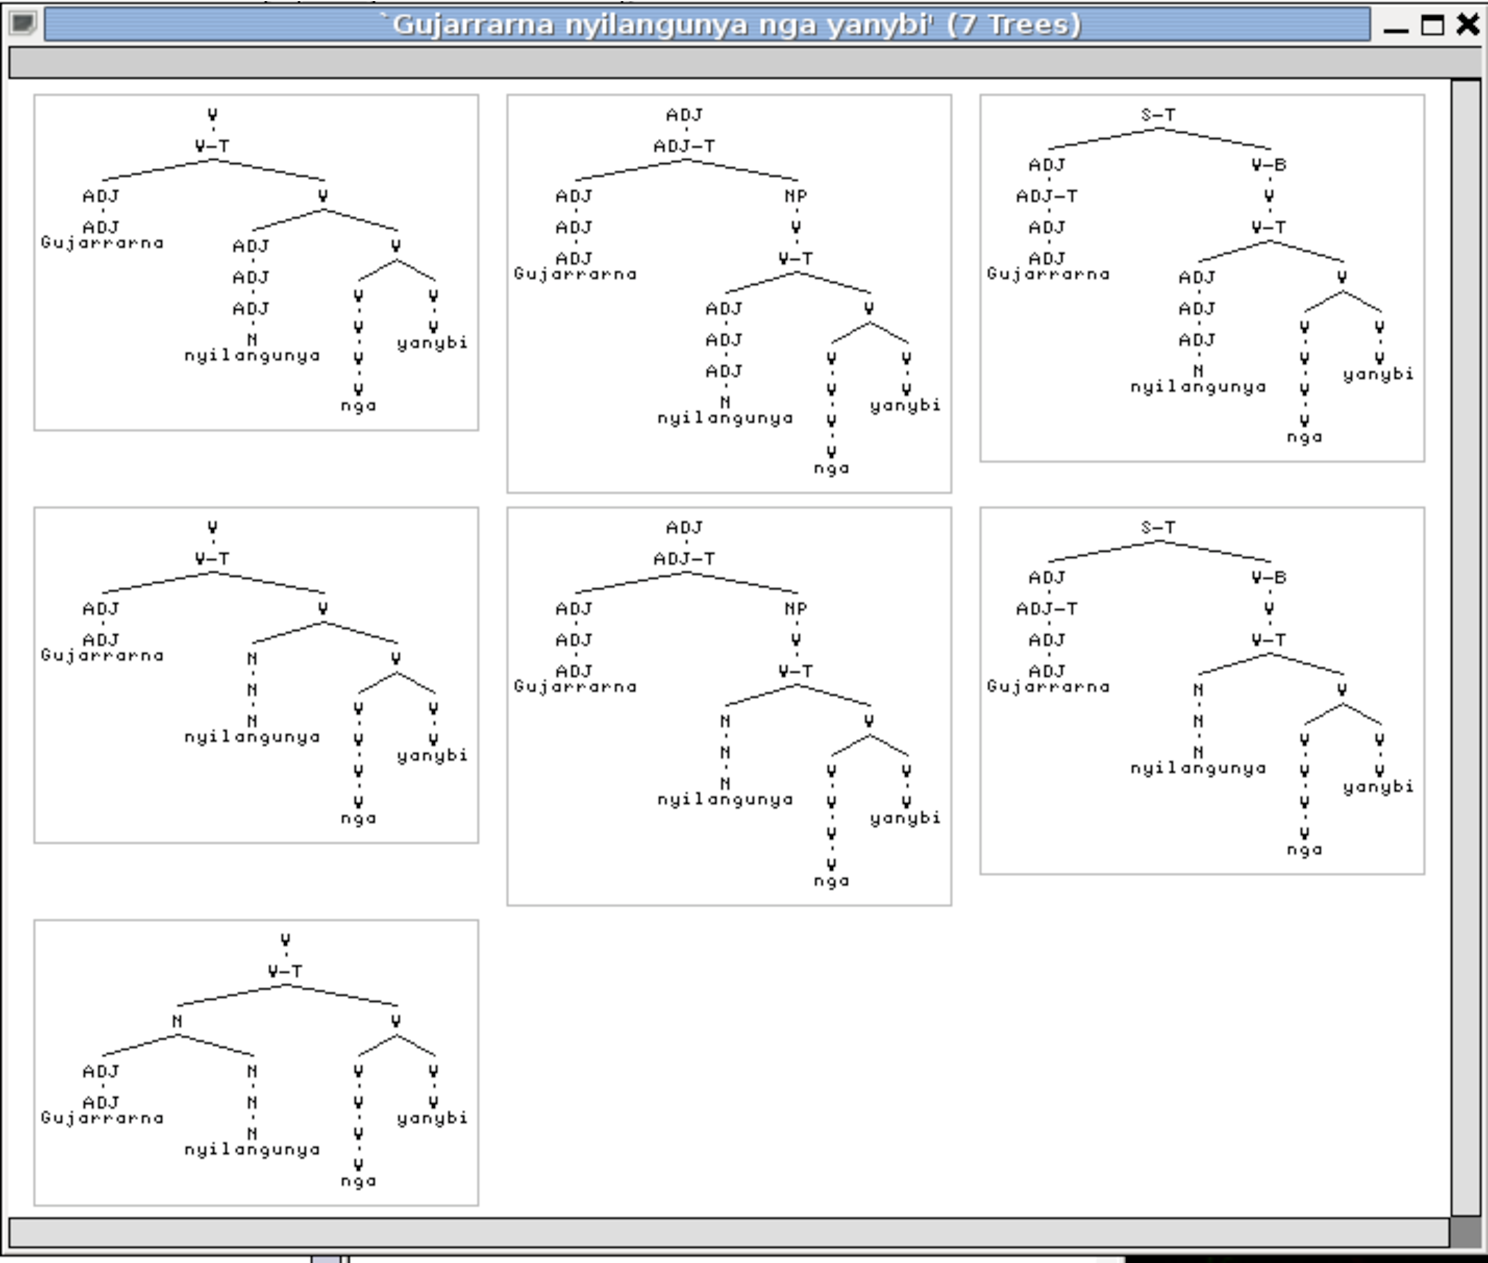
\includegraphics[width=5in]{trees}
\caption{Seven analyses of (\ref{ex:wmb1})}
\label{fig:lkb}
\end{figure}


Returning to the goals of integrating treebanks with electronic
descriptive grammars, the examples above highlight two important
points about implemented grammars and treebanks:
%
First, annotations derived from implemented grammars make explicit
ambiguity in natural language that speakers rarely notice and even
linguists often skip over, focusing only on the relevant reading of
the examples they are interested in.\footnote{One way that an
  implemented grammar can be incomplete is by licensing more analyses
  than are actually warranted for a string.  Not all ambiguity,
  however, is spurious ambiguity (i.e., involving
  grammatically ill-formed structures).  Any grammar with reasonable
  coverage will necessarily find multiple legitimate analyses of
almost any grammatical string it can analyze.  One of the lessons
of computational linguistics for linguistics is the sheer amount
of ambiguity in natural language \cite{Abney:96}.} 
In most cases, however,
only one of the analyses will correspond to a pragmatically plausible
reading.  Creating a treebank involves selecting that pragmatically
plausible analysis, as discussed further in \sref{sec:tb} below.
%
Second, implemented grammars and tools like the LKB are not enough
to meet the needs of grammar readers looking to use the annotations
in order to find relevant examples in a corpus.  A separate set of
tools is required which can take the output of the implemented
grammar and the treebanking process and provide search functionality.
Fangorn \cite{Gho:Bir:10} is a treebank search application that fills this 
need, as discussed further in \sref{sec:ts}.


% EB Say something about complementing ts with something that allows
% users to understand the analyses of the examples they find??



\subsection{Treebanks}
\label{sec:tb}

A treebank is a collection of natural language utterances annotated
with tree structures. Traditionally, treebanks have been created by
annotating the tree structures by hand, using a detailed annotation
guide. To speed up the process, the text may be first processed with
software tools such as a shallow parser or chunker, so that most of
the manual annotation consists of correcting and elaborating an
initial structure, rather than writing trees ``free-hand''.  The most
well-known treebank for English, the Penn Treebank
\cite{Mar:San:Mar:93}, was constructed in just such a fashion.  This
manual method of creating a treebank has many drawbacks. The most
forbidding is the amount of time required, even with the first
automatic pass, but there are other problems.  Validity of the
annotation is one: It is very difficult to maintain consistency when
annotating complex structures by hand, particularly when different
phenomena can interact in many ways. Another issue is the static
nature of these treebanks. Given the amount of time and money needed
to create them, once a treebank is annotated, it is rarely updated.
This means that out-of-date analyses are kept, even if later
investigation suggests a better hypothesis.

%% other treebanks, uses of treebanks, problems of hand-annotation
%% annotation guidelines, semi-automatic (ie hand-corrected)
%% staleness of annotations

\textit{Dynamic treebanks}, such as the Redwoods treebank \cite{Oep:Fli:Tou:04},
are produced by a newer method of treebank construction that uses an automatic
parser to process utterances according to an implemented grammar. Manual
annotation is still required, but in this case the annotator selects from the
possible trees produced by the grammar to nominate the most plausible (with
the option of rejecting all trees in case the grammar does not provide
a suitable analysis). Since the
annotator never edits tree structure manually, all annotations in the final
treebank are guaranteed to conform to the implemented grammar.  Aside from the
benefits of consistency and speed, dynamic treebanks also have the advantage of
being easy to update when the grammar changes, as described below.

For this type of treebank, once the text is parsed, the annotator selects the
correct tree by making a series of binary decisions based on so-called parse
discriminants \cite{Carter:99}.  
Figure~\ref{fig:tsdb} shows the interface of
the Redwoods treebanking tool used for this
process, with the trees displayed on the left, and the discriminants on the
right. Each discriminant represents a single aspect of analysis that occurs in
some trees, but not others. These differences could be in the syntactic or in
the semantic representation, where a syntactic discriminant consists of a
grammar rule and the portion of the sentence it is being applied to, and a
semantic discriminant describes a predicate and one of its properties or
arguments. An annotator can click on a discriminant and then select \textit{Yes}
to indicate that it is correct, or select \textit{No} to exclude any trees that
are compatible with this discriminant. Since there are many dependencies between
discriminants, selecting one can entail decisions for many others, meaning
that finding the correct tree may only require a small number of decisions.
These decisions are saved, and can then be used to (semi-)automatically update
the treebank after a change has been made to the implemented grammar. When the
text is re-parsed with the new version of the grammar, the old decisions can be
replayed where applicable, and then the annotator only needs to annotate items
that are still ambiguous after the old decisions have been applied.  In this
way, treebanks can be easily updated to reflect improvements in the grammar
without the need for complete (and costly) re-annotation.

\begin{figure}
\centering
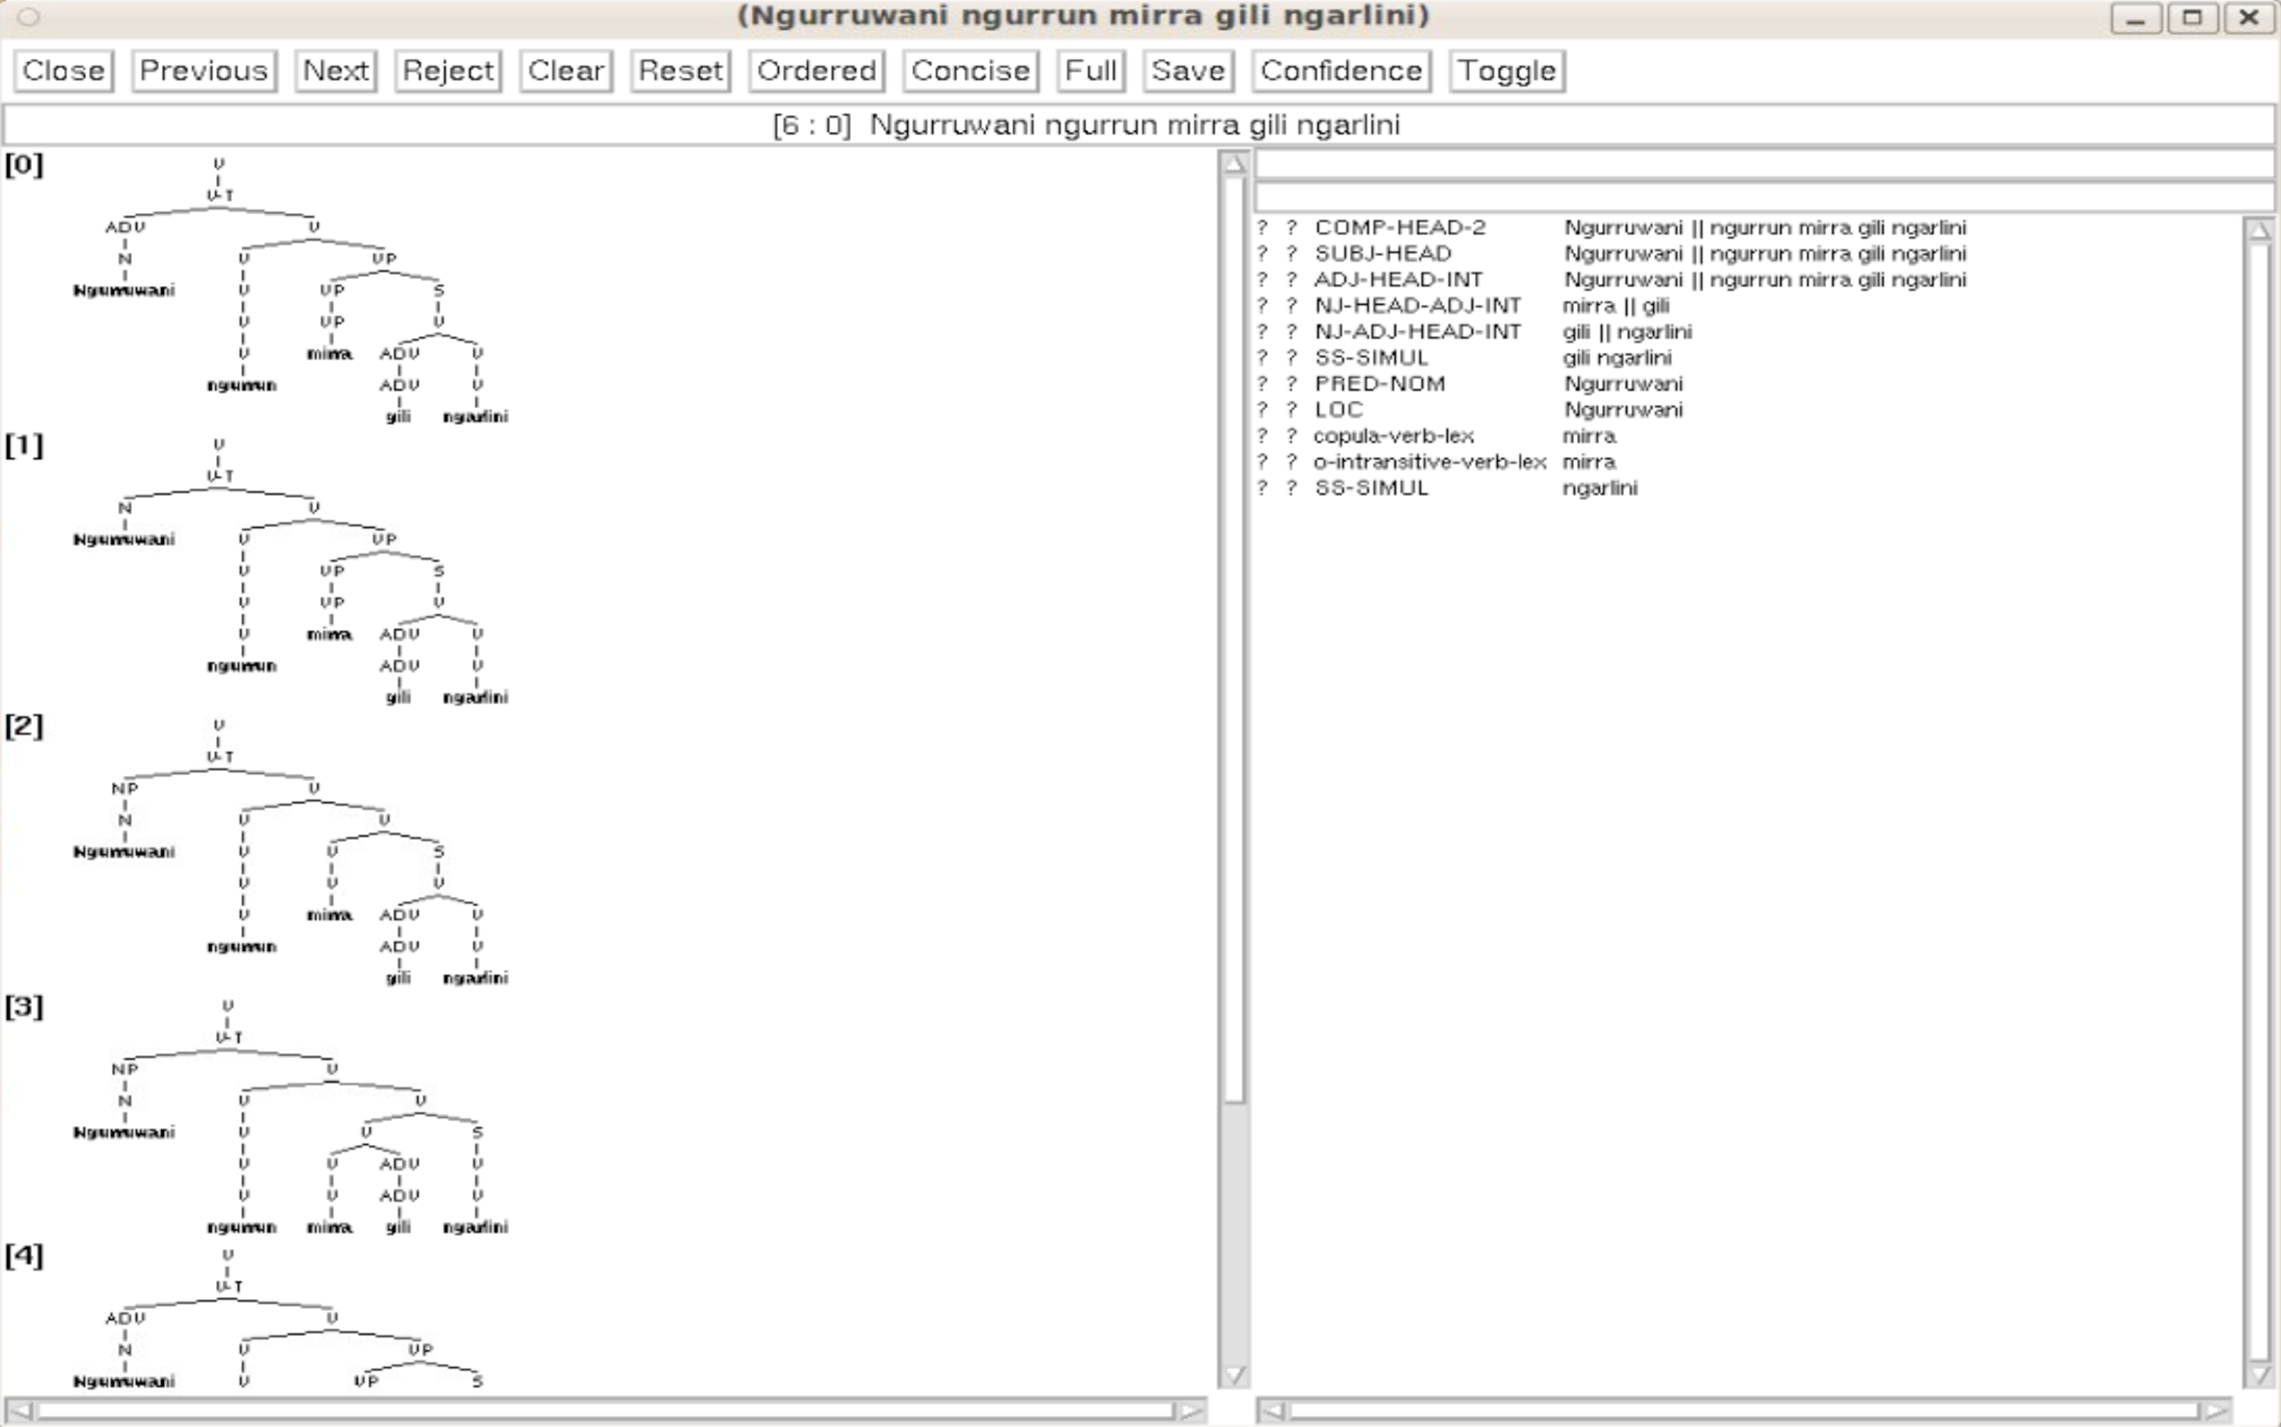
\includegraphics[width=6in]{treebanker}
\caption{Treebanking tool}
\label{fig:tsdb}
\end{figure}

In addition to their use in linguistic exploration, these treebanks can also be
used to build a statistical \textit{parse selection} model
\cite{Joh:Gem:Can:Chi:Rie:99,Tou:Man:Fli:Oep:2005}, which can be used to rank
parser output by probability.  While most human-detectable ambiguity requires
contextual information to resolve, the large majority of implausible analyses
can be ruled out on the basis of sentence-internal patterns.  These patterns are
probabilistic and very difficult to model with hand-written parse ranking rules,
but are well handled by the machine learning (pattern recognition) techniques
prevalent in computational linguistics.  For present purposes, parse selection
is of interest because it makes subsequent treebanking efforts easier.  By
learning characteristics of the trees selected as correct in a first round of
annotation, a parse selection model can be used by the parser to automatically
discard the most improbable analyses before the annotator sees them, speeding up
the annotation process.

\subsection{Summary}

In this section we have provided background on both implemented
grammars and treebanks, with the goal of sketching the technology
and methodology available.  The following section will build on this
to describe how treebanks can be used for linguistic research purposes.

\section{Using Treebanked data}
\label{sec:ts}

Treebank exploration is simplified by the use of specially designed
search tools.  These tools read in treebanked corpora and on request
provide instances of trees, similar to the one shown in 
Figure~\ref{fig:sent_tb}, that match the sought tree-pattern of linguistic 
significance from within a corpus.  Common features of
such tools are: a query language to specify the pattern of
interest and a user-interface to view the matching exemplars from
the corpora.

Treebank search tools such as TIGERSearch~\cite{Lez:Kon:00} and 
TGrep2~\cite{Roh:05} have been available for about a decade now.  
Only recently, however, with the development of Fangorn~\cite{Gho:Bir:10} 
has a solution become available which allows for efficient search 
over large-scale treebanks. 

\begin{figure}
\centering
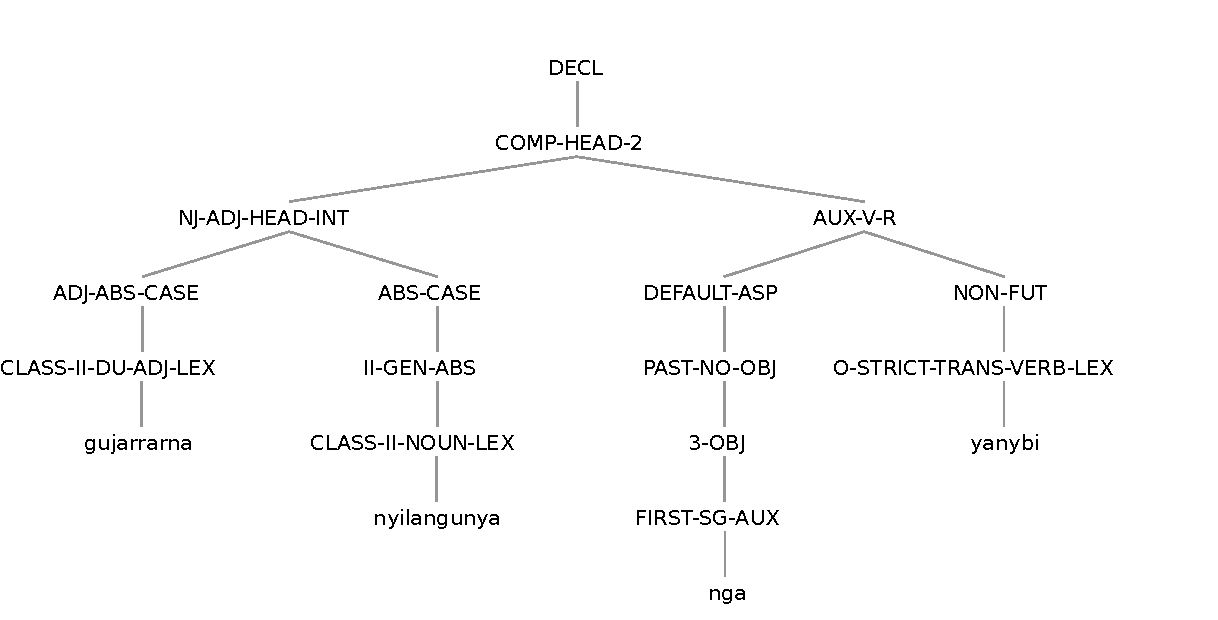
\includegraphics[width=5in]{sentencetreebank}
\caption{Treebank tree format for (\ref{ex:wmb1})}
\label{fig:sent_tb}
\end{figure}

\subsection{Fangorn}
\label{sec:tss}

Fangorn uses a path-based query language that is
a subset of the LPath query language \cite{Bir:Che:Sus:Lee:Zhe:06}.  For
a detailed comparison of different treebank query languages
see~\namecite{Lai:Bir:04}. 

Path query languages are used to specify tree nodes of relevance.  A
path is a sequence of required node labels together with operators
that state the relationship between consecutive labels.  In other
words, the path functions as a linear specification of nodes in trees
of interest. For example, one interesting property of Wambaya is that
modifiers can generally stand alone in argument positions
\cite{Nordlinger:98a}.  A linguist interested in 
sentences with this property might begin with a query like
(\ref{ex:qry1}), which finds all parses where a declarative clause
(label: {\small DECL}) has a complement of a verb realized by a modifier
(label: {\small HEAD-COMP-MOD-2}) below it.

\begin{exe}
\ex\label{ex:qry1}\small
\verb=//=DECL\verb=//=HEAD-COMP-MOD-2
\end{exe}

The operator \verb=//= in (\ref{ex:qry1}) is a \emph{descendant} operator. Table~\ref{tab:axis_ops} 
lists the different query operators in the Fangorn query language.
The operators have been categorized
into two types: horizontal and vertical, depending on whether they
specify dominance or sequential positional constraints. The semantics
of the vertical navigation operators are the same as their definition
in the context of a tree. Similarly, the names for the sibling operators 
are mnemonic for their functions. The
\emph{following} operator specifies that the node to the right of the
operator is temporally after the node to the left of the operator. The
\emph{immediately following} operator specifies that the leftmost descendant of
the node to the right is temporally immediately after the rightmost
descendant of the node to the left of the operator. The \emph{preceding} and
\emph{immediately preceding} operators are the inverse of \emph{following} and \emph{immediately
following}, respectively.

The first operator in the query specifies whether the query pattern
should appear at the root of the tree or anywhere in the tree. For
example, if query~(\ref{ex:qry1}) started with a \emph{child} operator rather
than a \emph{descendant} operator as it currently is, then, the pattern 
{\small \verb=/=DECL\verb=//=HEAD-COMP-MOD-2}, would match only if the topmost 
node of the tree was a declarative clause and that node had a 
{\small HEAD-COMP-MOD-2} under it.

Query (\ref{ex:qry1}) specifies a path consisting of two nodes,
however, paths could contain any number of operator-node pairs. Both
vertical and horizontal navigation operators can appear at any
position in the path. The only restriction is on the first operator in
the main path in the query. It has to be either a \emph{child} or a
\emph{descendant} operator.

An operator in a path specifies the relationship between the node
preceding and following it. In some cases, however, we would want to
specify more than one relationship at a single node. For example, 
we may want to modify query~(\ref{ex:qry1}) so that the head and 
complement positions are irrelevant, which means the node under the
declarative clause could be either {\small HEAD-COMP-MOD-2} or 
COMP-HEAD-MOD-2. Each of the two labels has a \emph{descendant}
relationship with the declarative clause {\small DECL}. Example (\ref{ex:qry2})
describes such a query.

\begin{exe}
\ex\label{ex:qry2}\small
\verb=//=DECL[\verb=//=HEAD-COMP-MOD-2 OR \verb=//=COMP-HEAD-MOD-2]
\end{exe}

Square brackets after any node in a path are called {\it filter expressions},
and can be used to indicate alternatives (a split into two or more possible
paths) or conjoined constraints on a node as shown in (\ref{ex:qry2}). 
%EB: Commenting out because this seems to repeat what is above.
%They could also be viewed as branches of the
%main path at a node, where the branches are the paths specified within
%the filter expression.  
The paths within a filter expression are
connected using logical operators AND, OR and NOT to add
flexibility to the constraints.  Further, since the paths within
filter expressions are themselves paths again, queries can have nested
filter expressions.

\begin{table}
\center{
\begin{tabular}{r l r l}
\multicolumn{2}{c}{\textbf{Vertical navigation}} & \multicolumn{2}{c}{\textbf{Horizontal navigation}} \\[3pt] 
descendant & \verb=//= & following & \verb=-->= \\
ancestor & \verb=\\= & preceding & \verb=<--= \\
child & \verb=/= & immediately following & \verb=->= \\
parent & \verb=\= & immediately preceding & \verb=<-= \\
 & & following sibling & \verb|==>|\\
 & & preceding sibling & \verb|<==| \\
 & & immediately following sibling & \verb|=>|\\
 & & immediately preceding sibling & \verb|<=| \\
\end{tabular}
}
\caption{Query operators and their symbols}
\label{tab:axis_ops}
\end{table}

Fangorn uses a web-based user interface, where the page
contains a search box and a result display area to show the matching
trees. A screen shot of the user interface for query~(\ref{ex:qry1}) 
is shown in Figure~\ref{fig:ts_web}.
The left-hand top corner of the display area shows the total
number of trees that match the query pattern in the corpus.  The first
page, showing 10 trees, is displayed by default. The user can choose
to navigate to other pages. Each tree may match the query pattern more
than once. Hence, the total number of matches within the tree and the
match currently being displayed is shown at the top of each
tree. Other matches within the same tree can be viewed using the
`$<$' and `$>$' buttons at the top of each tree. The trees are
minimally expanded to show the results in a concise manner, but
additional nodes can be expanded or collapsed in the display.  The
nodes that match the query are highlighted and joined by lines that
denote the operators between the nodes. Each matching tree can be
exported in either a bracketed format or as an SVG image identical
to how the tree is displayed on screen.

\begin{figure}[t]
\centering
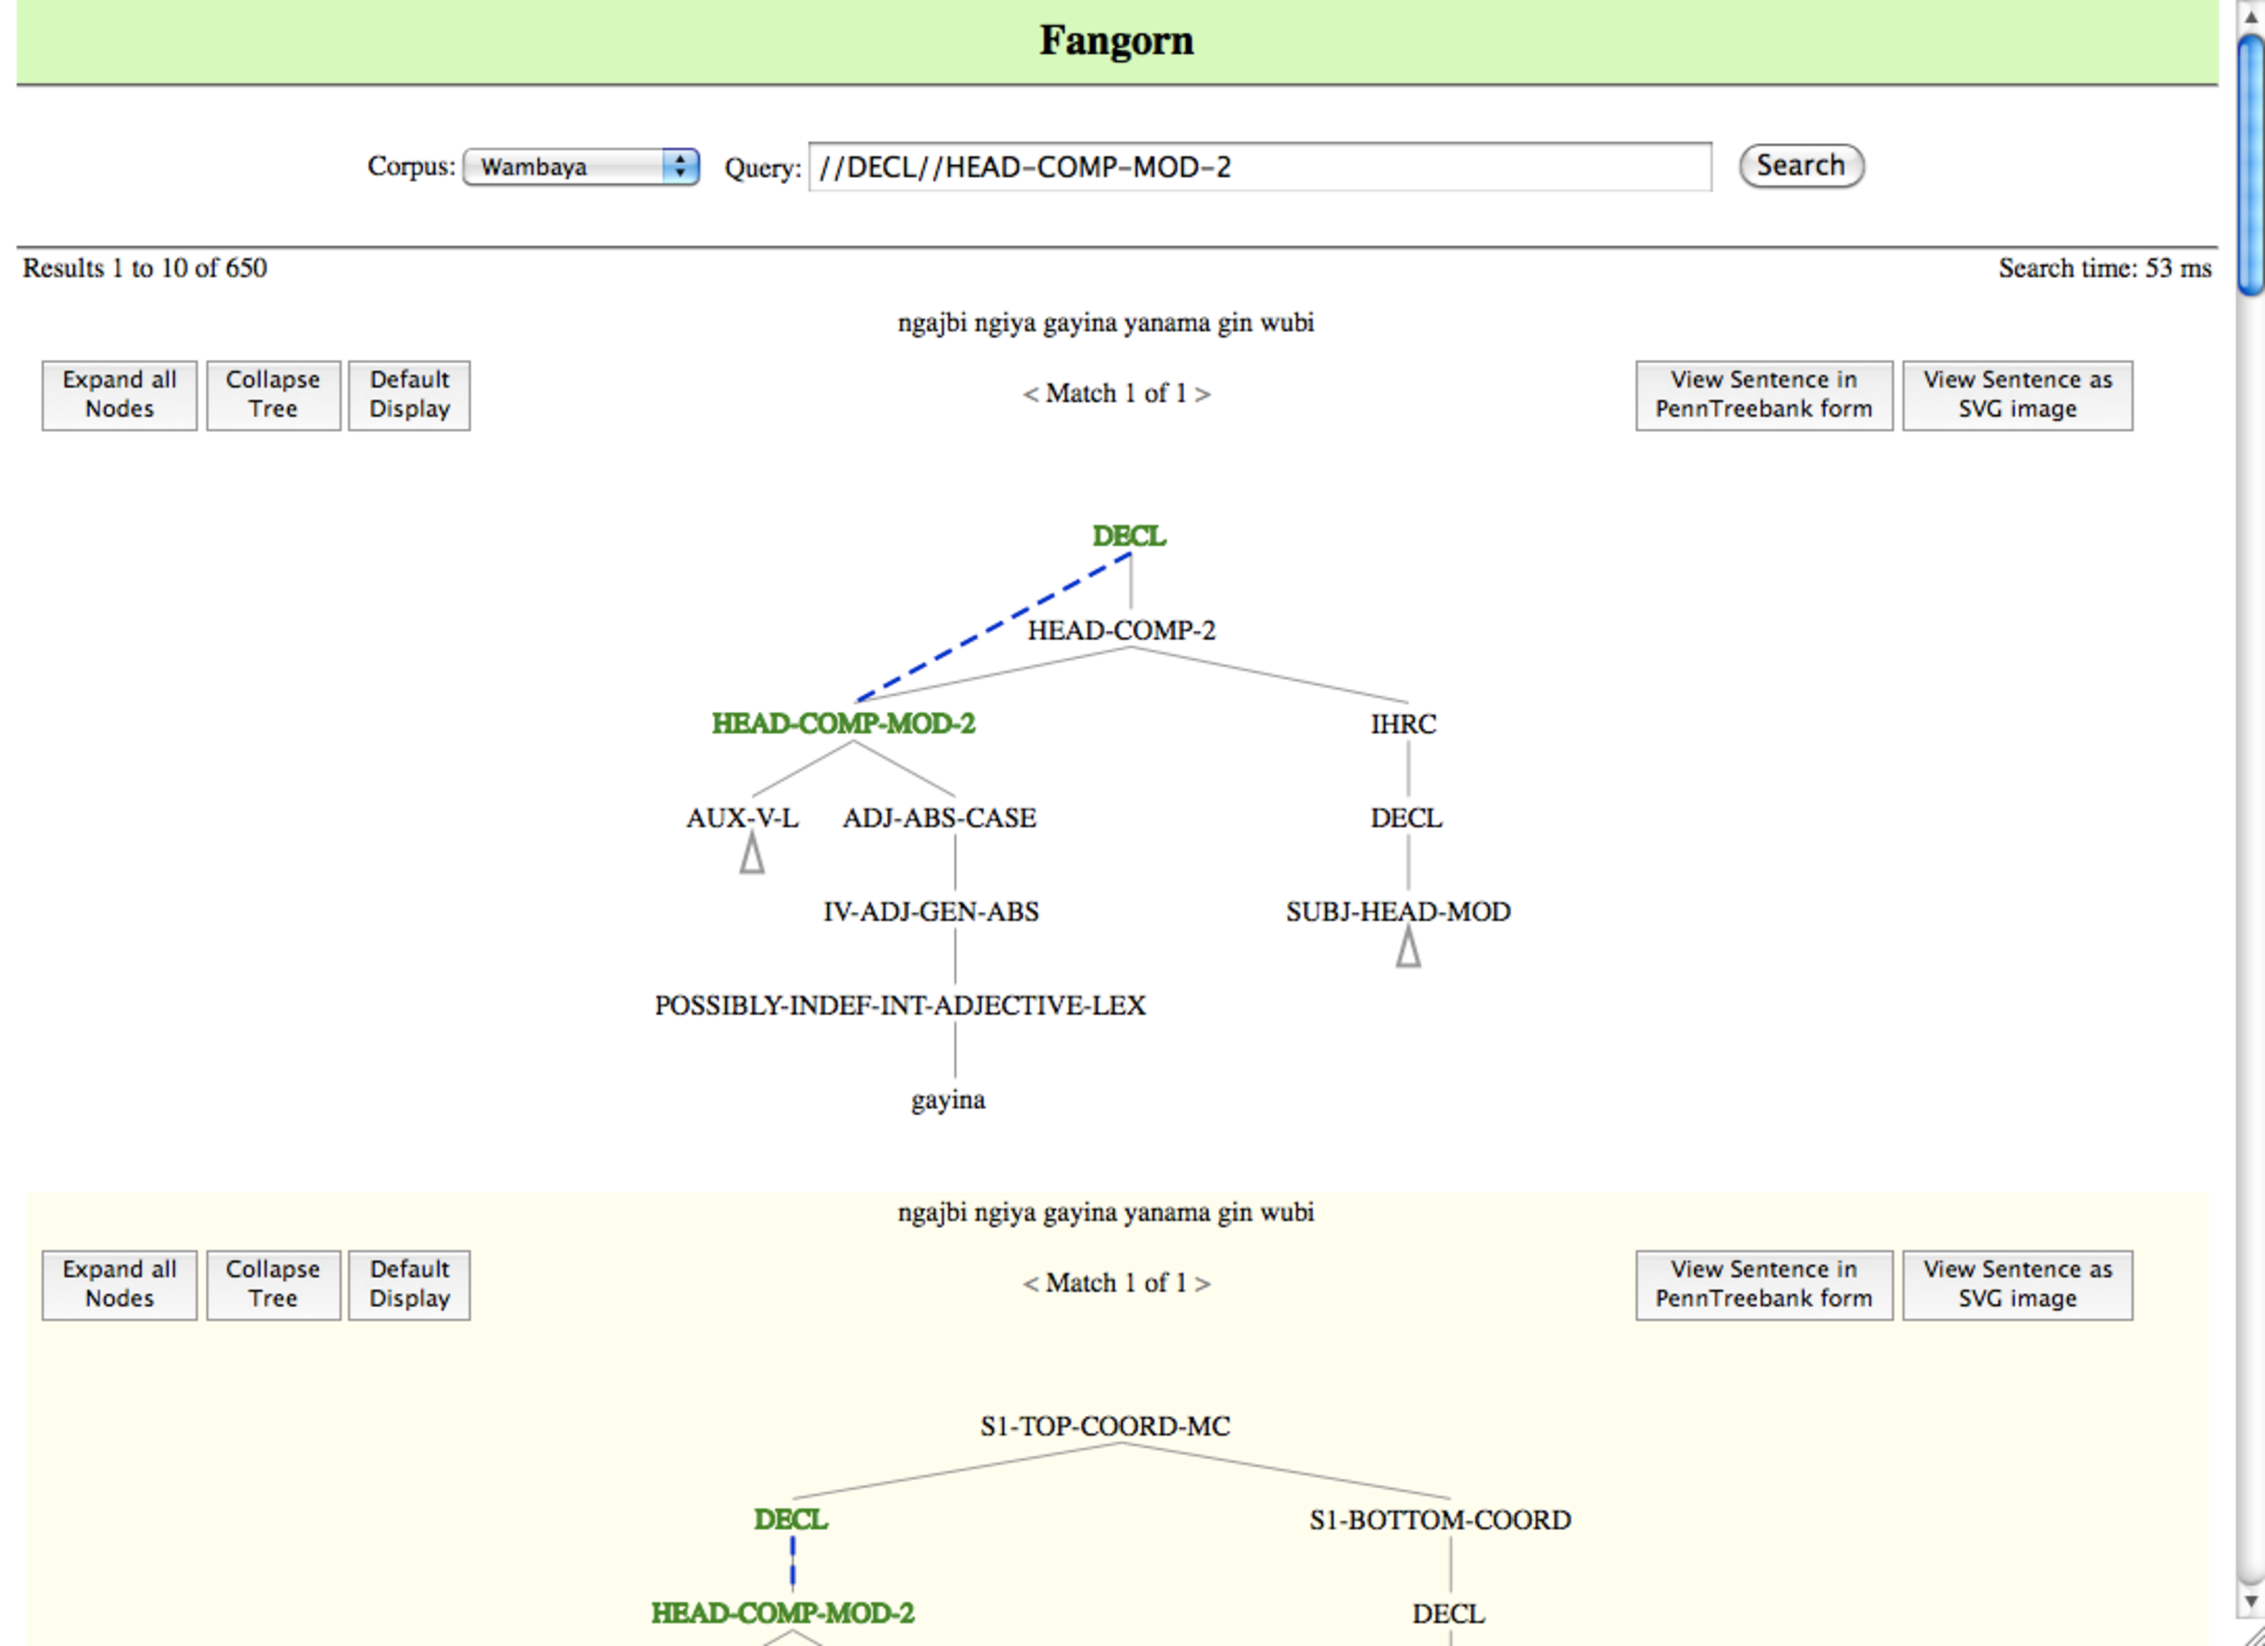
\includegraphics[width=6in]{searchinterface}
\caption{Fangorn's web interface}
\label{fig:ts_web}
\end{figure}

Fangorn can be used in a number of modalities, including
linguistic exploration, grammar engineering, and cross-linguistic
comparison.

Linguistic exploration can be viewed as a kind of ``exploratory data
analysis'' \cite{Tukey77}, whereby users query for particular
lexico-syntactic patterns in a given language, and, e.g., explore
the productivity of a construction, investigate the interactions between
different constructions, investigate the distribution/behavior of a
given construction across different domains (as instantiated in
different treebanks), or simply observe the distribution of given
lexical items in different syntactic contexts. \namecite{Resnik+:2005} is a good example of this sort of exploration using linguistic structure, although that work was not tied to a descriptive grammar.

Grammar engineers can use Fangorn to validate a new analysis, by
analyzing all instances of the given lexical rule or construction in
trees licensed by a grammar. Traditionally, Fangorn has been
applied to ``gold standard'' disambiguated trees. In indexing a larger
set of analyses licensed by the grammar (e.g., the top-500 analyses, as
selected by a parse selection model), however, it is possible to
retrieve all analyses in which a given pattern occurs, allowing the
grammar engineer to gauge whether an analysis is
adding spurious ambiguity. Fangorn can also aid in the education of grammar
engineers, in exploring how the analysis of a given construction is
manifested in syntactic trees, and comparing this back to the ``source
code'' for the analysis in the grammar files.

Finally, assuming a comparable label set between grammars of different
languages, it is possible to perform cross-linguistic queries to
compare, e.g., differences in right-node raising between English and
German in a data-driven manner. We come back to this briefly in Section \ref{sec:fangorn-fut}.



\subsection{Incorporating Treebank Search in Descriptive Grammars}

\namecite{Good:04} presents a vision of electronic descriptive
grammars as linked to searchable corpora, where exemplars chosen
by the author to illustrate particular phenomena can be linked
back to their original context, and additional examples can
be retrieved from the database.  We see the main benefit of treebanks
to descriptive grammars as enriching the range of ways in which 
examples can be retrieved.  

Treebank search can be incorporated into a descriptive grammar
in two different (and complementary) ways:  (i) The author of the grammar
can include specific ``canned'' queries at various points in order to allow
the reader to retrieve examples with properties relevant to
the discussion  (this would of course be in addition to providing
exemplars, as is usual practice); (ii) The treebank search interface
can be made available to the reader to input arbitrary queries
matching their own interests.  At present, Fangorn allows searching
over tree structures with the nodes labeled by the rule (phrasal or lexical)
or lexical type which licensed them, as well as over the words at
the leaves of the tree.  
%EB: FIXME: Say something about searching over node label
% abbreviations?  e.g., S, NP etc?
For the purposes of inclusion in descriptive grammars, it would be
useful to extend that search capability to include the other
annotations over the data (i.e., glosses and translations).  Longer
term, it would also be interesting to include searches over the
feature structures abbreviated by the tree structures, including
especially the embedded semantic representations.

The addition of ``canned'' queries will be relatively straightforward
(once the implemented grammar and treebank are built), and will most
likely be done in collaboration between the field linguist writing the
descriptive grammar and the grammar engineer developing the treebank
(cf.\ \sref{sec:gt}). The exact mechanism for making the canned queries
and associated results accessible to users of the grammars is open to
debate, but can potentially build off the work of
\namecite{Hashimoto+:2007} on lexical type documentation via
illustrative positive and negative examples.

Making the search interface itself useful to readers will require
documentation.  General documentation about the query language will be
applicable to all such treebank-enhanced grammars, but information about
the implemented grammar licensing each treebank will also be required.
The ``canned'' queries themselves will provide a useful part of this
documentation, serving as models for other similar queries.  In
addition, the documentation should include a glossary of all of the
labels in the treebanks (e.g., names of phrase structure rules, names of
lexical rules, names of lexical types, as well as category labels used).
Ideally, this glossary would include links to the relevant sections of
the descriptive grammar and thus be accessible from those sections as
well (following the links in the opposite direction).

\subsection{Summary}

In this section, we have given a brief overview of Fangorn,
how it can be used to formulate queries, and how those queries
could be used to assist readers of electronic descriptive grammars
in getting information from an associated treebank.  In the following
section we reflect further on how implemented grammars and 
treebanks can help fulfill the goals of descriptive and documentary
linguistics.

\section{Values and Maxims}
\label{sec:vm}

\namecite{Bir:Sim:03} structure a discussion of best practices
for creating portable (and thus useful and enduring) language
documentation around a series of value statements and maxims
that follow from those values.  \namecite{Nordhoff:08} picks
up that discussion with a particular focus on how values
identified by \citeauthor{Bir:Sim:03}
% as well as \namecite{Rice:06},
% \namecite{Noonan:06}, \namecite{Weber:06}, and \namecite{Cristofaro:06}
%EB should read those other sources and make sure
%this presentation makes sense.  Also, Nordhoff has two Rice 2006
%items in bibliography. Make sure this is the right one.
% Resolved: These don't use the value/maxim format, but they are
% relevant as sources for the suggestions in the maxims.  Removing
% the cites here and leaving them later.
influence the form of electronic descriptive grammars and inform the
design of software supporting the development of such resources.
\citeauthor{Nordhoff:08} is focusing in particular on those values
that are relevant to electronic grammars with non-linear
(i.e., graph-like) structure. 

In this section, we explore how the addition of treebanks to
electronic descriptive grammars can respond to some of those values,
with a particular focus on those that treebanks speak to, either
because they can enhance the ability of an electronic grammar to
fulfill a maxim or because they would in fact be problematic in some
way.  Following \citeauthor{Nordhoff:08}, we structure the discussion
according to the general areas of data quality, grammar creation (by
authors), and grammar exploration (by readers).  All of the maxims are
given in the consequent of a conditional with the associated value in
the antecedent, as in \namecite{Bagish:83}, the inspiration for
\quotecite{Bir:Sim:03} approach to discussing these
issues.\footnote{Except where noted, the antecedents and consequents
  are direct quotes from \namecite[308--318]{Nordhoff:08}.  Additional
  citations are provided when \citeauthor{Nordhoff:08} indicated other
  sources for the maxims.  Where there are multiple maxims for the
  same value statement, we have kept them as separate statements or
  merged them into one according to the most convenient structure for
  the present discussion. In \citeauthor{Nordhoff:08}'s terminology,
  `GD' stands for `grammatical description', i.e., what we are
  referring to here as an electronic descriptive grammar.}  This
discussion includes both near-term goals using existing technology as
well as longer-term possibilities.

\subsection{Data quality}

\begin{exe}
\ex {\sc Accountability:} If we value the application of the
scientific method, more sources for a phenomenon are better than
fewer sources (\citeboth[395]{Rice:06}, \citeboth[355]{Noonan:06}).
\end{exe}

This maxim is the most obvious win for treebank and treebank
search enhanced electronic grammars: If an electronic grammar
is paired with a database of interlinear glossed text (IGT), it
is already possible to search for some phenomena in that database.
The trees in a treebank make much more of the structure of the
sentences explicit than even the most meticulous IGT, and thus
treebanks make it possible to more easily find examples of a broader
range of phenomena (cf.\ \sref{sec:ts}).

\begin{exe}
\ex\label{ex:ou} {\sc Accountability:} If we value the application of the
scientific method, every step of the linguistic analysis should be
traceable to a preceding step, until the original utterance of the
speaker is reached.
\end{exe}

As noted above, an implemented grammar requires that the various
analyses it implements be integrated into a cohesive whole.  The
flip side of this is that every tree in a treebank represents several
levels of linguistic structure.  In grammars such as the Wambaya
grammar discussed in \sref{sec:wmb}, these include semantic, syntactic
and morphological analyses.  Thus, to the extent that the reader is
supported in exploring the trees, the trees themselves will help
ground semantic and syntactic analyses in previous steps.  The connection
between the morphological string and the original utterance will have
to be handled outside of the treebank, however.

\begin{exe}
\ex {\sc Accountability:} If we value the application of the
scientific method, the context of the utterance should be retrievable
\cite[450]{Weber:06}.
\end{exe}

\citeauthor{Nordhoff:08} discusses this one in terms of the communicative
context (who's speaking, to whom, with what goals, etc).  We assume that if this
information is documented in the database underlying the treebank, then it
should be accessible from the treebank as well.  However, another issue relating
to context arises for treebanks, namely the importance of preserving the
linguistic context.  All implemented grammars are in fact grammar fragments, and
thus will not necessarily have complete coverage over arbitrary samples of
naturally occurring text.  With reasonably mature grammars there are robustness
strategies \cite{Kie:Kri:Car:Mal:99,Rie:Kin:Cro:Max:Kap:02} that potentially allow for partial analyses
in a treebank, but these are unlikely to be applicable or desirable in this
application.  Thus, a treebank associated with an electronic descriptive grammar
will necessarily have gaps, i.e., sentences which are not assigned any trees. In
order to preserve the linguistic context of the examples which are assigned
trees, and which thus can be retrieved with Fangorn, it will be
important to maintain links between the treebank and the underlying dataset.

\begin{exe}
\ex\label{ex:act} {\sc Actuality:} If we value scientific progress, a
GD should incorporate provisions to incorporate scientific progress.
\end{exe}

\citeauthor{Nordhoff:08} notes descriptive grammars are never
finished.  In the same way, implemented grammars also always have room
to grow.  It is a major benefit of the Redwoods approach
to treebank construction \cite{Oep:Fli:Tou:04} that treebanks can be
cheaply and rapidly updated when the grammar that produced them has
been changed.  Thus modern treebanking methodology makes it possible
for electronic grammars with treebanks to rise to this maxim.

\begin{exe}
\ex {\sc History:} If we value the recognition of the historic evolution
of ideas, the GD should present both historical and contemporary
analyses \cite[360]{Noonan:06}.
\end{exe}

The same software that supports the creation of treebanks
({\itsdb}, \citeboth{Oep:Fli:98}) allows for detailed comparisons
between treebanks based on different grammar versions.  The primary
purpose of these comparisons has been to allow grammar engineers
to explore the impacts of various changes they have made to the
grammar, in terms of which items (sentences) are assigned different
(or more or fewer) analyses by one version of a grammar than 
another.  It is possible that this same software could be adapted
to facilitate the exploration of the evolution of analyses either of particular examples
in an implemented grammar, or of classes of examples.  Doing so in a way
that would make it informative for linguists who are not grammar
engineers would, however, require significant additional user interface
effort. 


\subsection{Grammar creation}

The particular maxims that \citeauthor{Nordhoff:08} proposes under
this heading are specific to the design of a grammar-authoring platform
that supports the creation of electronic descriptive grammars, and
therefore don't speak to the creation of implemented grammars. Accordingly,
instead of reviewing \citeauthor{Nordhoff:08}'s maxims, we have
proposed some of our own that concern the creation of implemented
grammars (and thus treebanks), but relate to the same set of values.

\begin{exe}
\ex\label{ex:cc} {\sc Assistance}: If we value speed of creation
and comparability (across grammars), we should seek to provide
means to assist linguists in rapidly creating comparable implemented grammars.
\end{exe}

This is in fact the goal of the Grammar Matrix project
\cite{Ben:Fli:Oep:02,Ben:Dre:Fok:Pou:Sal:10}.  
The Grammar Matrix provides a common core grammar, which defines
things such as the format of semantic representations (using Minimal
Recursion Semantics \cite{Cop:Fli:Pol:Sag:05}), an implementation of
semantic compositionality, and general types of rules and lexical
entries.  In addition, the Grammar Matrix provides a set of libraries
of analyses of cross-linguistically variable phenomena.  These libraries
are developed on the basis of a review of the typological literature,
though of course are not assumed to be comprehensive: the project
always anticipates the addition of new options within a library, as well 
as changes to the core grammar.
The Grammar Matrix is described further in \sref{sec:gt} below.

\begin{exe}
\ex\label{ex:cr} {\sc Creativity}: If we value the individual mind's expressive
abilities, support for creating implemented grammars should
not preclude the linguist exploring alternative analyses in the
implemented grammar.
\end{exe}

The Grammar Matrix is in a sense analogous to the prose templates
that \citeauthor{Nordhoff:08} proposes as part of a grammar authoring
platform.  Both make it easier to create a linguistic resource
(descriptive grammar or implemented grammar), in terms of coverage
of phenomena and in terms of compatibility with the relevant set of
tools.  At the same time, these aids can also have the adverse effect
of limiting creativity or biasing analyses towards those anticipated
by the creator of templates/libraries of analyses.  Compared to prose
templates, Grammar Matrix libraries are more difficult to create
(represent a larger investment of time and effort) and are likely also more limiting.  Both
of these effects follow from the fact that implemented grammars 
require all of their component analyses to interact.  On the one hand,
the grammar engineers constructing the libraries must design them
carefully to be interoperable with all of the options of all of
the other libraries \cite[Ch.\ 2]{Drellishak:09}.  On the other
hand, a linguist attempting to develop an alternative analysis for
one phenomenon will find herself hemmed in to a certain extent by
the decisions made in the analyses of other phenomena.

Nonetheless, we believe that grammar engineering provides a net
benefit for analysis exploration because computers can be harnessed to
test the analyses against large data sets
\cite{Bender:08,Ben:Fli:Oep:11}.  Thus even though it can require
non-trivial work to implement alternative analyses, their relative
advantages and disadvantages can be empirically explored
\cite{Bender:10}.  Recently, \namecite{Fokkens:11} has been investigating
the potential of `metagrammar engineering', or the development of
systems that provide not only implemented analyses of varying
phenomena, but in fact multiple analyses per variant.
\citeauthor{Fokkens:11} argues that this will alleviate the risks of
implemented grammars being shaped by the order in which phenomena are
analyzed.

\begin{exe}
\ex\label{ex:collab} {\sc Collaboration:} If we value the potential
for faster progress when multiple investigators collaborate, we should
develop methodologies and tools which support
collaboration.\footnote{\citeauthor{Nordhoff:08} provides a different
  value statement under the heading collaboration: ``We value
  collaboration and the recognition of the respective contributions of
  the collaborators'' (p.\ 302).  We do not disagree with that value
  statement, but find the one provided in (\ref{ex:collab}) more
  relevant to the present discussion.}
\end{exe}

As will be discussed further in \sref{sec:gt}, grammar engineering for
language documentation is an excellent example of the kind of project
that thrives on collaboration, in this case between one or more field
linguists and one or more grammar engineers.  The grammar engineering
work is dependent on the field work and cannot proceed without data
collection, transcription and analysis done by the field linguist.  At
the same time, grammar implementation allows the hypotheses generated
by both the field linguist and (eventually) the grammar engineer to be
systematically tested against the collected data.  Tools which would
facilitate this kind of collaboration include those which help field
linguists to produce consistent and well-formatted IGT, on the one
hand, and those which make the resulting implemented grammar available
for interactive inspection (such as web-interfaces to parsing and
generation algorithms) on the other.

%% EB: I don't really have anything to say about this one.  Just
%% skip it? Talk about version control?
%% \begin{exe}
%% \ex If we value the safety of data,
%% \end{exe}

\subsection{Grammar exploration}
\label{sub:grammar_exploration}

\begin{exe}
\ex {\sc Ease of finding:} If we value ease and speed of retrieving
the information needed, a GD which has a table of contents, an index
and full text search is preferable.
%EB the following is also in Nordhoff, but we don't really have
%anything to say to it:
%, and a GD that does not require internet
%access is preferable.
\end{exe}

Fangorn is an extremely valuable tool for finding information
within a treebank, provided that readers know how to formulate
the queries they are interested in.  We envision embedding pre-formulated
search queries within the electronic prose grammar (as links that
retrieve additional examples from the database, for example).  An
annotated index of these queries could be a useful source of information
for a linguist seeking to formulate additional queries.  

A second question is how to link back to the relevant parts of the
grammar from the trees in the treebank.  Ideally, each phrase
structure rule, lexical rule and lexical type in the implemented
grammar would be annotated with the phenomenon or phenomena that it
implements.  With such annotations, a reader could move from the tree
assigned to a particular sentence to the relevant discussions in the
prose grammar.  The exact means of encoding these annotations is an
issue for future work.  However, we note here that linking to a
particular prose descriptive grammar is probably a more tractable
problem than producing a general index of a stand-alone implemented
grammar.


\begin{exe}
\ex\label{ex:ff} {\sc Individual reading habits:} If we value the individual
linguist's decisions as to what research questions could be
interesting \cite[402]{Rice:06}, a GD should permit the reader to
follow his or her own path to explore it and a short path between
two related phenomena is better.
\end{exe}

\begin{exe}
\ex\label{ex:mn} {\sc Manipulation:} If we value portability and reusability of
the data, the data presented in a GD should be easy to extract and
manipulate.
\end{exe}


The key issue regarding individual reading habits, according to
\namecite{Nordhoff:08}, is that some readers will be asking how a
particular function is realized within a language, while others will
be interested in the function(s) associated with a particular form.
In this context, the fact that Redwoods-style treebanks (as described
here) include semantic representations is a key asset.  While at
present, Fangorn only applies over syntactic structures, it
can conceivably be extended to searches over semantic structures as
well as combined syntactic/semantic queries.  

Furthermore, if the implemented grammar is made available along with the
treebank, it, too, becomes a tool for both form- and function-based
exploration, greatly enhancing the ways that the data can be
manipulated.  For form-based exploration, the reader can send strings to
the grammar for parsing.\footnote{The grammar will return multiple
  analyses in many cases, but if a parse selection algorithm
  is trained on the treebank, those analyses can be ranked
  by their predicted likelihood.}  For function-based exploration, the
reader would want to use a generation algorithm (e.g., that included
with the LKB \cite{Car:Cop:Fli:99}).  Generation algorithms that
work with Grammar Matrix-derived grammars take as input Minimal
Recursion Semantics representations \cite{Cop:Fli:Pol:Sag:05}, which
cannot easily be written by hand.  However, the Grammar Matrix is
compatible with the LOGON machine translation (MT) infrastructure
\cite{Lon:Oep:Ber:04}.  While it would take additional work to produce
an MT system (notably the writing of a transfer grammar), this could in
principle be done.  In that case, within the coverage of the MT system,
readers could submit sentences in the other language of the MT pair and
retrieve strings in the language being documented.  The trees associated
with those strings could then point into the descriptive grammar (as
above).\footnote{Note that for {\sc quality assessment} (\ref{ex:qa})
  and {\sc accountability} (\ref{ex:ou}), strings returned by the
  generator would need to be flagged according to whether they match
  strings in the collected data or in fact represent generalizations
  based on the hypotheses encoded in the grammar.}


\begin{exe}
\ex {\sc Familiarity:} If we value ease of access, a GD that is similar
to other GDs known to the reader is better.
\end{exe}

Here we must acknowledge that treebanks and implemented grammars
will not be immediately familiar to linguists on first encounter,
and there is work to be done to make them more accessible.  However,
once a linguist has become familiar with one such resource, that
familiarity should be readily transferable to another one constructed
in a similar fashion.  This once again underscores the importance
of tools in promoting standardization (cf.\ (\ref{ex:cc})).

\begin{exe}
\ex {\sc Guiding:} If we value an informed presentation of the data,
the GD should present the data in a didactically preferred way
\cite[401]{Rice:06}.
\end{exe}

\begin{exe}
\ex {\sc Ease of exhaustive perception:} If we value the quest
for comprehensive knowledge of a language \cite[162]{Cristofaro:06}, the
readers should be able to know that they have read every page of the grammar.
\end{exe}

%FIXME: (Before camera ready.) Double check Cristofaro to see if that
%makes sense.

Implemented grammars are intricate objects (full of interconnections)
and the field of grammar engineering is still struggling with
developing best practices for documenting them.  It is unlikely that a
treebank or implemented grammar would assist in the ordering of
information or the creation of paths through a prose descriptive
grammar or with ease of exhaustive perception.  However, by embedding
links to Fangorn in that grammar, the prose descriptive
grammar could become a very effective guide to the implemented grammar
(to the extent that the analyses in the implemented grammar all
directly map to analyses in the prose grammar).

\begin{exe}
\ex {\sc Relative importance:} If we value the allocation of scarce
resources of time to primary areas of interest, the relative importance
of a phenomenon for (a) the language and (b) language typology should
be retrievable (\citeboth[2]{Zaefferer:98}, \citeboth[355]{Noonan:06}).
\end{exe}

There are of course many different ways of defining importance
of phenomena.  If one takes a quantitative approach, a treebank can
be a useful tool in exploring such things. Assuming we have an index
linking grammar rules and lexical entries to phenomena described in the
prose grammar, it should be possible to quantify the text
frequency of each phenomenon.  Likewise, the number of rules/entries
in the grammar which are indexed to the phenomenon would give a 
sense of the degree to which that phenomenon interacts with others.

Regarding cross-linguistic relevance, in the long term, the Grammar
Matrix project has the potential to provide this information:  If
there are many grammars constructed on the basis of the Grammar
Matrix and its libraries (the ``customization system''), we will
be able to quantify the relative prevalence of each choice in each
library, as well as co-occurrence tendencies between the choices.
In addition, it is in principle possible to detect whether 
specific analyses in an implemented grammar remain consistent with
the starting point provided by the Grammar Matrix or required changes.\footnote{Of course, there is also always the influence of the grammar engineer
(cf.\ {\sc creativity} (\ref{ex:cr}) above): a grammar could differ
from the analyses provided by the Grammar Matrix because those analyses
did not work for the language in question, or because the grammar
engineer chose to explore alternatives.}

\begin{exe}
\ex\label{ex:qa} {\sc Quality assessment:} If we value indication of
the reliability of analyses, the quality of a linguistic description
should be indicated.
\end{exe}

The development of an implemented grammar is a fairly stringent test
of the quality of linguistic analyses.  It is not of course the case
that implemented analyses are necessarily correct.  However, with
implemented analyses it is possible to tell whether analyses of
multiple phenomena are consistent with each other and also the extent
to which the analyses collectively account for the available data (cf.\
Good's concept of {\it internal coverage} (this volume)). \nocite{Good:tv}
That is, the quality of a treebank and its underlying implemented
grammar can be partially assessed in terms of the number of examples
in the underlying database which are assigned a tree.

In order for this assessment to reflect on the prose descriptive
grammar which is the basis of the implemented grammar, at least two
points need to be made explicit: (1) the extent to which the analyses
in the implemented grammar are faithful to the descriptive grammar, and
(2) the extent to which the implemented grammar incorporates all of the
analyses in the descriptive grammar.  That is, the descriptive grammar
could be very comprehensive, but if the implemented grammar does not
include analyses for every phenomenon treated in the descriptive
grammar, treebank coverage will be poor.

Using treebanks to assess the quality of individual analyses
is somewhat more problematic.  The same indexing of implemented grammars
that was suggested for measuring the relevance or importance of
particular phenomena could also be used to estimate the success
of their analysis in implemented grammar.  However, these two
factors are confounded:  A highly central or important phenomenon with
a poor analysis would appear to be relatively unimportant, since the
poor analysis could lead to poor coverage for the sentences with
the phenomenon.  Thus what is called for is an independent way to
measure the frequency of phenomena (perhaps based on interlinear
glossed text alone) and then compare that to the measurements taken
over the treebank.

So far this brief discussion has considered grammar/treebank
quality only in terms of coverage, or the ability to find a correct
analysis for any given example.  Another important measure of grammar
quality, however, is ambiguity: Grammars or analyses which are
underconstrained will produce many spurious analyses.  These will not
be apparent in the final treebank, as they are discarded in the manual
annotation step.  However, the maxim in (\ref{ex:qa}) suggests that the
degree of ambiguity found by the grammar underlying the treebank
should be reported.  In addition, it is straightforward to quantify the
extent to which particular rules and lexical entries contribute to
ambiguity.\footnote{Note, however, if a particular rule is prone
to adding ambiguity, that may not be the fault of the analyses of
the phenomena it currently implements (and thus is indexed for) but
rather the analysis of some other phenomenon which should involve
constraints on that rule but does not.}

Finally, we note that in the development of treebanks for descriptive
grammars, the correctness of a tree is determined by comparing the
semantic representation associated with that tree to the translation
and gloss provided for the example.  Thus to the extent that quality
issues in the descriptive grammar affect the quality of the glossing,
these issues will be masked in measures involving the treebank.

\begin{exe}
\ex {\sc Persistence:} If we value citability \cite[14]{Bir:Sim:03},
in order to facilitate longterm reference, a grammatical description
should not change over time.
\end{exe}

As \nocite{Bir:Sim:03} Bird \& Simons and \citeauthor{Nordhoff:08} note,
the solution to the conflict between this maxim and the one
in (\ref{ex:act}) is to take snapshots which can be the anchors
for citations.  The addition of treebanks to electronic descriptive
grammars makes this somewhat more difficult as the versions between
the treebank (and implemented grammar) on the one hand and the
prose descriptive grammar on the other need to be synchronized.
This is perfectly possible, however, with proper planning.

\begin{exe}
\ex {\sc Tangibility:} If we value the appreciation of a grammatical
description as a comprehensive aesthetic achievement, a GD that can 
be held in the hand is better.
\end{exe}

Implemented grammars and treebanks are only valuable as
computational artifacts, and thus will only be the sort of
thing that can be held in the hand when hand-held devices
are powerful enough to run them.  That said, the addition of
an implemented grammar should not get in the way of the production
of the associated descriptive grammar as book.  In practical terms,
any links to treebank searches that are embedded in prose
chapters should be either stripped or made non-disruptive.
In addition, any links in a printed volume must be stable
links that will continue to function as long as possible.

\begin{exe}
\ex {\sc Multilingualization:} If we value the interest of every human
in a given language, especially interest from the speakers of the language
in question, a GD should be available in several languages, among others
the language of wider communication in the region where the language
is spoken \cite[433]{Weber:06}.
\end{exe}

There are two primary ways in which implemented grammars and treebanks
can respond to this maxim.  The first is to be designed to be able to
incorporate and display glossing of the primary data into multiple
different languages.  The second (and longer term) method is through
the machine translation possibilities discussed in reference to the
values {\sc individual reading habits} (\ref{ex:ff}) and {\sc
  manipulation} (\ref{ex:mn}) above.  It is possible in principle to
set up multiple MT systems between a language being described and
different languages of wider communication.  Furthermore, while there
is additional work required for every language pair, each additional
language pair should require less set up work than the first.

\subsection{Summary}

Our purpose in this discussion has been twofold: On the one hand, by
reflecting on values and maxims, we have proposed a series of design
desiderata for the incorporation of treebanks in electronic
descriptive grammars.  On the other hand, we hope to have provided
arguments in favor of the value of treebanks and implemented grammars
to the enterprise of language documentation and description, and
clarified the role that they can play.

%% In summary, it appears that treebanks will be particularly helpful
%% in achieving the goals associated with the values of ...

The incorporation of treebanks into descriptive grammars is possible
on the basis of existing technology, including technology supporting
grammar development, parsing, generation, treebank creation and
maintenance and treebank search.  This is sketched in the following
section.  The preceding discussion makes it clear that achieving the
full potential of the integration will rely on further advances in a
few areas. These include: methodologies and software support for
indexing components of implemented grammars, support for rapid
deployment of machine translation, and user-interface improvements to
make implemented grammars and the analyses they assign to strings more
accessible to non-grammar engineer linguists.


\section{Getting there}
\label{sec:gt}

In the previous sections, we have presented the idea of augmenting
electronic descriptive grammars with treebanks and reflected on how
doing so will help descriptive grammars fulfill the values that 
have been articulated for them.  This section addresses the feasibility
of creating implemented grammars and treebanks and discusses the
resources that are available to assist in the creation of such
resources as well as future directions.

\subsection{The Grammar Matrix}
\label{sec:gm}

Building implemented grammars can be expensive and time-intensive.
The English Resource Grammar (ERG) has been under development since 1994,
and now achieves 62-94\% verified coverage over naturally occurring
corpora from a variety of genres \cite{Flickinger:11}.\footnote{The
low end of that spectrum relates to fairly technical corpora,
including technical manuals and chemistry papers.  Verified coverage
over 80\% is more typical.}  The example of the ERG shows that
this kind of grammar and treebank construction is indeed possible,
but it also suggests that it might be too expensive to be applied
in context of language documentation, as envisioned here.

We contend that it is not, for several reasons.  First, a grammar does
not have to be comprehensive, or even approach the ERG's level of
coverage, in order to be useful.  Even a partial treebank would begin to
yield benefits for linguists searching for examples (though it will be
important to make clear the extent to which the treebank covers the
total corpus, cf.\ {\sc quality assessment} (\ref{ex:qa}) above).
Secondly, it is unfortunately the case that language documentation
projects rarely approach a range of genre diversity in the data
collected that compares to the range of genres the ERG has been tested
against.  A smaller genre range means a more tractable problem for
grammar engineering.  Finally, much of the effort that has gone into the
ERG represents solutions to problems that are not in fact
English-specific, but more general contributions to efficient, implemented \hpsg
parsing.

This last point is the motivation for the LinGO Grammar Matrix
\cite{Ben:Fli:Oep:02,Ben:Dre:Fok:Pou:Sal:10}.  Specifically, the
Grammar Matrix aims to facilitate the development of implemented
grammars in languages without such resources by curating and making
available advances from the ERG and other broad-coverage grammars
developed in the DELPH-IN\footnote{\url{http://www.delph-in.net/}}
consortium, most notably the Jacy Japanese grammar \cite{Sie:Ben:02}
and the German grammar \cite{mueller_s-kasper_w00}.  The Grammar
Matrix consists of a core grammar, shared by all language-specific
grammars derived from it, a series of libraries of analyses of
cross-linguistically variable phenomena, and a ``customization
system'' which allows users to select from among those analyses by
filling in a web-based questionnaire.  

The core grammar includes definitions (constraints) that are
hypothesized to be cross-linguistically useful.  The customization
system pairs these with more specialized constraints on the basis of
information collected through the questionnaire. The questionnaire
elicits from a linguist-user typological information of varying
granularity: for example, major constituent word order (including
various flexible word order options), the means of expression of
negation, the range of cases (if any) marked on core arguments, the
possibility of dropping each core argument and information about its interpretation when
dropped.  It also allows users to define classes of lexical items and
morphological rules.  Morphological rule definitions include morpheme
forms,\footnote{These are expected to be regularized underlying forms.
  We follow \namecite{Ben:Goo:05} in advocating for separate
  components for morphophonological and morphosyntactic analysis.
  Various tools exist for creating morphophonological analyzers,
  including XFST \cite{Bee:Kar:03}.} morphosyntactic and
morphosemantic features (case, tense, etc.)\ associated with the
morphemes, and ordering and co-occurrence constraints with other
morphemes (including stems).

This strategy of code reuse necessarily involves taking analyses
developed on the basis of well-studied languages and applying them to
lesser-studied languages.  However, the Grammar Matrix project is
explicitly data-oriented in its approach to cross-linguistic
universals and cross-linguistic variation.  With regards to the
constraints provided in the core grammar, these are treated as working
hypotheses only, ready to be revised (or more precisely made variable
and moved into the libraries) when we encounter languages which
present counter-examples.  The methodology of grammar engineering
allows us to empirically test the applicability of analyses and
determine when an analysis really won't work.  Furthermore, our
library development methodology begins with a review of the
typological literature so that we are working with the most
comprehensive possible view of the range of variation in the world's
languages as we develop the libraries of analyses.

The work on Wambaya cited above \cite{Bender:08a} provides 
a case-study in the feasibility of grammar engineering for language
documentation.  The grammar produced is approximately an order
of magnitude less complex than the English Resource Grammar.
% FIXME: Try to quantify that in terms of types/leaf types/rule instances/lines of code?
Nonetheless, it provided interesting coverage over both the
exemplars cited in \namecite{Nordlinger:98a} and a naturally occurring
text used to test the grammar's ability to generalize beyond the
data used in grammar development.  It was possible to achieve this
level of coverage so rapidly thanks in part to the restricted
range of data being considered (relatively short sentences, relatively
little genre variation) but more importantly thanks to the analytical
work done by Nordlinger.  It is in some ways easier to implement analyses
presented in a descriptive grammar than to work from intuitions about
one's own language combined with analyses gleaned from the theoretical
linguistic literature.  In other words: the original descriptive
work (done in this case by Nordlinger) is the hard part.  When this is
done thoroughly and done well, the grammar engineering is relatively
straightforward.

\subsection{Treebanking Support}

Once an initial version of an implemented grammar has been written, building an
\textit{undisambiguated} treebank is an automatic process that can be easily
initiated using the suite of tools available. Treebanking, the process of
selecting the most plausible tree using discriminants (see
Section~\ref{sec:tb}), requires further effort, but much less than manually
annotating the data. 
%% add something about using the examples from the descriptive data to help?
%%also something about who does the treebanking
While treebanking will always require a human annotator if we wish to
maintain quality, there is some work on automatic methods to help make
treebanking easier.  One method that has proved successful in previous
experiments is to rank the discriminants so as to present those most
likely for an annotator to select at the top of the
list. \namecite{Zha:Kor:10} showed that treebanking speed could be
improved by using the annotation logs of their treebankers to build a
statistical model that ranked the discriminants in the order which an
individual treebanker would be likely to select them. Another method,
called blazing \cite{Tan:Bon:Oep:Fuj:05,MacKinlay+:2011b}, uses
supplementary information available about the text to partially
pre-annotate. In this work, the authors used pre-existing annotations of
parts of speech (in the case of \citeboth{Tan:Bon:Oep:Fuj:05}) or phrase
structure trees (in the case of \citeboth{MacKinlay+:2011b}) to
automatically mark some discriminants, leaving the annotator less
decisions to make, and also found increases in treebanking speed.  Rather
than requiring external information, a third strategy would be to use
all the analyses produced for all items to learn trends in the
analyses. While this information is noisy, the trends from the less
ambiguous items inform the decisions to be made for the more ambiguous
items and this partial information can be used to automatically learn a
probabilistic ranking function to rank all analyses. In this way, we can
prune improbable analyses and in the process accelerate treebanking
\cite{Dridan:Baldwin:2010}.

%%A third strategy is to take advantage of the constrained nature
%%of the grammar, and generate all analyses for a given item. By selecting
%%more plausible analysis from these via heuristics or lexical type
%%assignments, it is possible to automatically learn a probabilistic
%%ranking function to rank/prune analyses licensed by the grammar
%%\cite{Dridan:Baldwin:2010}. This can potentially prune improbable
%%analyses from the parse forest, and in the process, accelerate
%%treebanking, without the requirement for a pre-existing treebank.



%% Not sure if we need this section.  Are there further
%% details on how to make a treebank/how to set it up for
%% treebank search that would be relevant here?
%%
%% RD: I've had a go, but this might be more confusing than beneficial - too 
%% much background required to make the points clear?

\subsection{Future Work on Fangorn}
\label{sec:fangorn-fut}

%% linking, searching across parallel annotations (different layers)
%% looking for examples in another language - GOLD labels?

At present, Fangorn has a query language that is sufficient to express
simple queries using paths and filter expressions. However, for more complicated 
queries with multiple logical operators in a filter expression, allowing
braces to group terms would make queries more expressive.
For example, let us consider query~(\ref{ex:qry2})
and add further conditions that require the search to match only those parses 
where the complement of the verb is realized only by a modifier and not by a
nominal head. We would now have to exclude trees which have a {\small HEAD-COMP-2}
or {\small COMP-HEAD-2} label underneath the declarative clause. Query~(\ref{ex:qry2})
would have to be reframed as shown in (\ref{ex:qry3}). If the grouping of elements,
using braces, were allowed we could rewrite (\ref{ex:qry3}) as (\ref{ex:qry4}), 
which is not only more concise, but is also easier to read. 

\begin{exe}
\ex\label{ex:qry3}\small
\verb=//=DECL[\verb=//=HEAD-COMP-MOD-2 AND NOT \verb=//=HEAD-COMP-2 AND NOT \verb=//=COMP-HEAD-2 OR \verb=//=COMP-HEAD-MOD-2  AND NOT \verb=//=HEAD-COMP-2 AND NOT \verb=//=COMP-HEAD-2]
\end{exe}
\begin{exe}
\ex\label{ex:qry4}\small
\verb=//=DECL[(\verb=//=HEAD-COMP-MOD-2 OR \verb=//=COMP-HEAD-MOD-2) AND NOT (\verb=//=HEAD-COMP-2 OR \verb=//=COMP-HEAD-2)]
\end{exe}

Another potential means of grouping terms within a filter expression
would be to take advantage of the types declared in the grammar behind
the treebank, which group together sets of rules.
For instance, there are grammar types in Wambaya grammar, shown in (\ref{ex:gram}) (cf.\ Figure~\ref{fig:hcp}), that 
match the two elements of the filter expression in (\ref{ex:qry4}). Replacing elements in (\ref{ex:qry4}) with their grammar type would allow us to further refine the query to (\ref{ex:qry5}). 
The search tool could itself perform the substitution of grammar types with actual labels 
rather than expect the user to input expanded queries. For this to work, Fangorn 
has to be aware of grammar types and expand them prior to execution.

\begin{exe}
\ex\label{ex:gram}
{\small\tt head-2nd-comp-mod-phrase: \{ head-comp-mod-2, comp-head-mod-2 \}}\\
{\small\tt wmb-head-2nd-comp-phrase: \{ head-comp-2, comp-head-2 \}}
\end{exe}

\begin{exe}
\ex\label{ex:qry5}\small
\verb=//=DECL[(\verb=//=HEAD-2ND-COMP-MOD-PHRASE AND NOT \verb=//=WMB-HEAD-COMP-2ND-COMP-PHRASE]
\end{exe}

The current version of Fangorn operates over the abbreviated tree
structures that are used for presentation purposes. The abbreviated trees are
sufficient to distinguish between competing analyses, but they don't expose all
the information that a user might wish to search for. As mentioned in
Section~\ref{sub:grammar_exploration}, the semantic information embedded in the
tree would provide a useful mode of querying. This provides some interesting
challenges in determining the best way to represent semantic information so that
it can be queried, since a tree structure is not a natural representation for
semantics.  We are currently pursuing two different approaches to this problem:
either trying to find a natural way to represent the semantic information we
have in a treelike form, or alternatively, looking for an intuitive extension of
the query language that would allow querying over a more appropriate 
%graph-like?
representation.

Being able to query the syntax and semantics separately provides different views
and avenues of access to the same data. Likewise, other levels of annotation
that exist, such as glosses and translations, could be useful in finding the
examples that a user requires. A simple extension to Fangorn is planned
to allow different annotation levels to be aligned, so that it is possible to
search using one representation and see how the same data is analyzed at a
different level. A more complex extension would allow a query to filter using
multiple levels of annotation, for example using semantic restrictions to filter
a syntactic query. This extension could require extensive changes to the query
language for a fully general solution, but it might be possible to achieve most
of the desired capabilities by designing a means of specifying metadata about
annotations both within the treebank and in the query language.
%FIXME: Before final version.  I think this point still needs to be elaborated
%a bit more.

Another area of future work for Fangorn is the mapping of labels
onto a cross-linguistic label set, e.g.\ based on GOLD
\cite{Farrar:Lewis:2007}. This would involve aligning individual grammar
rules, lexical rules and lexical types onto the GOLD ontology to mark
features such as verb transitivity, noun case and clause illocutionary
force, while preserving the language-specific rule types and/or more
familiar node labels (e.g., {\small NP} and {\small VP}) as are 
currently used. This would significantly enhance cross-linguistic
treebank search, as the label set would be harmonized to a much greater
extent than occurs using the ``native'' label set for individual
grammars.


\subsection{Virtuous Cycles and the Montage Vision} 

The Wambaya case study described above was an exercise in post-hoc
grammar engineering: The implemented grammar wasn't developed until a
decade after the original field work was complete, and sadly, the
language lost its last fully fluent speakers in that time.  The process
of grammar engineering always raises further questions about the data
(as no grammatical description is ever complete), and the Wambaya case
study suggests that collaborations between grammar engineers and field
linguists could be very fruitful:\footnote{We would like to emphasize that nothing in the
  preceding discussion requires that the grammar engineering and field
  work be done by the same person, and in fact it seems unlikely that many
  people would have the skill sets required for both. Going further,
  it seems like grammar engineering would be a less than efficient use
  of the time of someone who has the skills to do original fieldwork.}
While a considerable amount of data collection and analysis has to
take place before grammar engineering can get off the ground, if the
field linguist is still working with speakers when the grammar
implementation work begins, there is the potential for a feedback loop
that speeds up and strengthens the descriptive work.

The Montage project \cite{Ben:Fli:Goo:Sag:04} envisioned a software
environment which integrated tools for the production of IGT,
electronic descriptive grammars and implemented grammars.  The IGT and
the descriptive grammar would inform the implemented grammar, and even
possibly be input to a system that could automatically create a
partial implemented grammar. The implemented grammar would in turn
feed IGT and descriptive grammar development by locating interesting
exemplars (through Fangorn\footnote{Note that this could even
  be done before the manual annotation step of the treebank
  construction process: the treebank search tools described above work
  equally with undisambiguated sets of trees.}), highlighting
possible inconsistencies in glossing, and testing out analyses.

The Montage project itself was never funded, but nonetheless there is progress
in the direction of this vision, including:

\begin{itemize}
\item Collaborative annotation and descriptive grammar authoring environments,
including GALOES \cite{Nordhoff:07}, TypeCraft \cite{Bee:Mih:09} and Digital Grammar \nocite{Drude:11} (Drude, this volume)
% Check Drude cite to see if it's relevant
% Resolved: Yes, looks relevant.
\item The Grammar Matrix customization system (\citeboth{Ben:Dre:Fok:Pou:Sal:10}, cf.\ \sref{sec:gm})
\item The Redwoods methodology for dynamic treebank construction (\citeboth{Oep:Fli:Tou:04}, cf.\ Section~\ref{sec:tb})
\item Treebank search using Fangorn (\citeboth{Gho:Bir:10}, cf.\ \sref{sec:tss})
\item Machine learning algorithms that learn typological properties
from IGT (e.g., \citeboth{Lew:Xia:07})
\end{itemize}

The Grammar Matrix makes it feasible to create interesting implemented
grammars for languages without large computational resources, while the Redwoods methodology
makes treebank development practical. Fangorn makes the
treebanks useful as resources for readers of descriptive grammars.
The longer term goal of semi-automatic grammar implementation is
supported by the Grammar Matrix and the work of \namecite{Lew:Xia:07}
which suggests that it might be possible to learn answers to questions
like those in the Grammar Matrix questionnaire on the basis of
(sufficiently large) sets of IGT (with sufficiently meticulous
glossing).

\section{Conclusion}

In this paper we have presented a vision of how electronic descriptive
grammars can be enriched with implemented grammars and treebanks, and
described how such a vision is supported by current technology as well
as what future developments could add further value.  Following the
discursive approach of \namecite{Bir:Sim:03} and
\namecite{Nordhoff:08}, we have explored the ways in which implemented
grammars and treebanks can help to meet the values and associated
maxims proposed regarding producing the most useful possible language
resources.  To our knowledge, no such treebank-enhanced descriptive
grammar yet exists, but we hope to see them emerge through the
collaboration of field linguists and grammar engineers.

%FIXME before final version
%\section*{Acknowledgments}

% NSF Grammar Matrix grant
% Fangorn funding?
% Conference audience
% Reviewers
% who else?

\bibliography{paper}
\bibliographystyle{robbib}

\end{document}
